\documentclass{idc_msc}

\title{Advanced Topics in IP Networks \\\large Out of bailiwick project}
\date{Last edited \today}
\author{Ron Aharoni\texorpdfstring{ - 300028065}{}, Steven Karas\texorpdfstring{ - 328620984}{}, Phillip Kaplan\texorpdfstring{ - 324478403}{}}
\AtBeginDocument{\maketitle}
\AtEndDocument{\vfill\bibliographystyle{plain}\bibliography{biblio}{}}

\begin{document}

\paragraph{Collaboration Statement}
  % I worked alone and only with course materials.
  We worked alone and referred to sources cited inline and in the references section, and well as the course materials.
  % I collaborated on this assignment with (students), got help from (others), and referred to (citations to sources other than class material).

  % General guidelines (for all HWs in this course):
  % • Each student should submit an individual solution.
  % • Do your best to cope with the problem set by yourself.  It is OK to work in groups and to discuss your solution with other students, but these discussions should be verbal. You are not allowed to copy/dictate/etc.
  % • It is perfectly OK to skip some questions. There is no mandatory submission of all questions or all HWs in this course.
  % • For clarifications or any other help, you are welcome to use the course forum in Piazza
  % • Your work should include a header stating everyone you worked with to solve the homework and every other source you have used.
  % • Submit your work electronically via the course Moodle page. Submit your solution in PDF format. Other formats (DOC, ZIP, etc.) are not be accepted. 
  % • In case you scan a handwritten solution, make sure the pages are properly ordered and oriented, the text is in focus, the contrast between the text and the background is high, and the resolution is such that the page width fits a standard computer screen. The whole solution should be submitted in one pdf file.
  % • Failing to meet any of the submissions requirements may result in point deduction or even your submission not being graded.

\section{Abstract}

\section{Background}

% TODO: fill in background on DNS and nameservers and glue records
% TODO: fill in background on bailiwick concept and in-bailiwick servers and out-of-bailiwick servers

DNS in broad strokes works by translating human-friendly textual names into IP addresses that can be used to send traffic to a server.
DNS is organized into a hierarchical tree with a single entity responsible for each branch in the tree.
For example, the root of the tree is managed by ICANN, and each of the top level domains underneath are managed by various registries.\\
Glue records are critical to the proper functioning of the DNS system\cite{rfc1033}. However, improper use of glue can leave a domain susceptible to various security vulnerabilities. Here we attempt to analyze the use of certain best practices by domain owners on the internet, specifically the prevalence of “out of bailiwick” glue records.

\subsection{Related Work}
In “The Availability and Security Implications of Glue in the Domain Name System” \cite{2016arXiv160501394W} Zheng Wang discusses the necessity of glue records to the proper functioning of DNS along with the implications of current practices in terms of both availability and security. He presents the ability of known mitigation techniques to prevent certain classes of cache poisoning attacks on DNS.
The cache attacks he discusses were originally presented by Dan Kaminsky in his presentation “Blackops2008 – it's the end of the cache as we know it”.
Wang additionally discusses the implications of DNSSEC and attacks on it, and whether bailiwick checking is relevant if the records are secured.

\subsection{Bailiwick definition}

A bailiwick for DNS purposes is defined\cite{rfc7719} as:

\begin{quote}
In-bailiwick:

      (a) An adjective to describe a name server whose name is either
      subordinate to or (rarely) the same as the zone origin.  In-
      bailiwick name servers require glue records in their parent zone
      (using the first of the definitions of "glue records" in the
      definition above).

      (b) Data for which the server is either authoritative, or else
      authoritative for an ancestor of the owner name.  This sense of
      the term normally is used when discussing the relevancy of glue
      records in a response.  For example, the server for the parent
      zone "example.com" might reply with glue records for
      "ns.child.example.com".  Because the "child.example.com" zone is a
      descendant of the "example.com" zone, the glue records are in-
      bailiwick.

   Out-of-bailiwick:  The antonym of in-bailiwick
\end{quote}

\section{Data}

We downloaded the Majestic Million\cite{MajesticMillion} on January 18th, 2019.
This is a list of the top one million sites ranked by the number of subnet that link to them, collected and published by Majestic.com.
From these, we constructed a list of 1,000,878 domains and domain prefixes to check for out of bailiwick glue records.

\subsection{Data Quality}

From some randomized sampling of the domain list, some of the domains are listed because of links to subdomains, whereas others were included despite being subdomains of others in the list (e.g. plus.google.com and google.com both appear on the list). Additionally, not all of the domains returned valid records (e.g. ns1.example.com as their NS record), were valid domains (e.g. http://163), or had any records at all (NXDOMAIN).

To deal with these issues we decided that the correct approach was to do our analysis on zones rather than on domains. Domains that we did not consider to represent valid zones:
\begin{itemize}
  \item Domains that returned “NX Domain”
  \item Domains that returned an SOA record (e.g. plus.google.com)
\end{itemize}

Out of the million initial domains we constructed a list of 1,000,878 domains and domain prefixes by using all of the possible subdomains. We did this with a simple script. Out of the generated domains, 964039 turned out to represent valid zones.

\subsection{DNS record collection}

We used a BIND server configured as a recursive resolver to query the records for the domain list.
We run a small pipeline in parallel\cite{Tange2011a} to do this quickly.

% In parallel to building the code to query the DNS directly, we requested access to the zone files for all the gtlds, including .com and .name, and several ccTLDs that were listed.
% This will allow us to ensure authoritative data.

% \paragraph{.DE ccTLD zone file policy}

% \href{https://www.denic.de/en/faqs/general-information/#faq-154}{DENIC}, the authoritative registry for the .DE ccTLD hold a strict policy of not sending the zone file to any third parties.

\subsection{Data Collection}

DNS queries
To perform the DNS queries, we used dig. Dig is a command line tool for querying the domain name system. We used the following command to fetch the name server records for all domains:
\begin{verbatim}
dig [domain] @127.0.0.1 NS
\end{verbatim}
Where the localhost flag instructed dig to use the local resolver.
Since we were limited largely by the round trip time of serially sending queries, to speed up the process we used the parallel utility running 20 queries at any given time.

We used a BIND server configured as a recursive resolver to query the records for the domain list.
We constructed and sent our queries using dig in a parallel \cite{Tange2011a} pipeline to quickly gather the data:

\begin{verbatim}
cat majestic_all_possible_domains | parallel -j 20 -- dig {} @127.0.0.1 NS | 
  gzip > dig.output.gz
\end{verbatim}

After less than 6 hours all of the queries had been completed and the data stored in a text summary file.

\subsection{Data Analysis}

using Python3 to parse the zone files and gather statistics. Graphs were plotted using pandas and matplotlib.
We set up a short pipeline to collate the unsorted results against the original ranked list:
\begin{verbatim}
	tail -n+2 raw_results.csv | sort -t, -k1 | pv -l | cat > sorted_results.csv
tail -n+2 majestic_million.csv | sort -t, -k3 | pv -l | cat > sorted_majestic.csv
join -t, -o 2.1,0,1.2,1.3,1.4,1.5 -1 1 -2 3 sorted_results.csv sorted_majestic.csv | 
  sort -t, -k1 -n | pv -l | cat <(echo $'Majestic Million Rank,Domain,
    Num NS records,Num glue records,Num out-of-bailiwick glue,Num loose-out-bailiwick glue') 
      - > collated_results.csv
\end{verbatim}
We then used pandas and matplotlib to generate plots showing the CDF of having out-of-bailiwick glue records.

% TODO: we should check the quality of the dataset before doing the analysis

% https://singaporedatacompany.com/blog/how-many-domain-names-are-unused
% https://dofo.com/

% certificate transparency for certs - to enumerate all public websites

% anecdote: feedio.net is errored out, but seems to have subdomains used for copyrighted content streaming.

\section{Evaluation and Discussion}

\begin{table}
\begin{tabular}{l|cc}
 & & \\
 \hline
 Number of domains & 1,000,879 & \\
 NXDOMAINs & 26,678 & \\
 Number of empty domains & 65,708 & \\
 Number of NS records & 2,476,318 & \\
 Number of glue records & 3,156,909 & \\
 Number of improper glue records & 0 & \\
 Out of bailiwick glue & 3,078,764 & \\
 Loosely out of bailiwick glue & 1,600,449 & \\
\end{tabular}
\end{table}

\subsection{Prevalence of third party providers}

\begin{table}
\begin{tabular}{l|cc}
 Provider & Domains & \\
 \hline
 ns.cloudflare.com & 218,747 & \\
 domaincontrol.com & 129,789 & \\
 worldnic.com & 65,400 & \\
 myhostadmin.net & 61,948 & \\
 dnspod.net & 45,038 & \\
 hichina.com & 43,271 & \\
 dnsmadeeasy.com & 40,619 & \\
 dns.com & 24,208 & \\
 registrar-servers.com & 23,821 & \\
 googledomains.com & 23,705 & \\
\end{tabular}
\caption{Domain count for 10 most popular providers}
\end{table}

% TODO: describe and cite code on github for actual collection and analysis

% TODO: present collected statistics

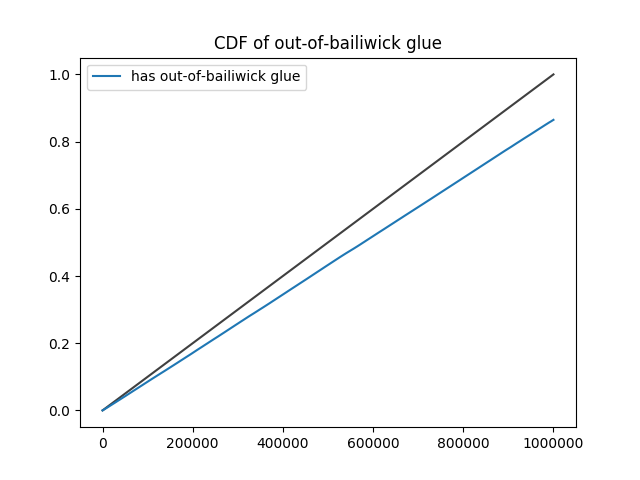
\includegraphics[width=15cm]{cdf.png}


% TODO: discuss possible future directions
% IDEA: collect data from other locations (azure, residential ISPs, etc)
% IDEA: cover potential solutions to the security issues

\section{Conclusion}
Our results clearly show that use of out of bailiwick glue is a widespread practice. This appears to be due to the prevalence of name servers being hosted by third party providers such as GoDaddy or Cloudflare. Third party name server hosting is largely a desirable situation, as requiring smaller web hosts to have their own nameservers would add significant relative complexity to their network and require additional expertise, and would therefore provide additional attack surface ripe for exploitation by a determined attacker. The better way to deal with this problem is likely to make use of DNSSEC, which is much more resistant to the types of attacks analyzed in the works we discussed.

\end{document}
